\documentclass[10pt]{article}
\usepackage{amsmath}
\usepackage{graphicx}
\usepackage{float}
\usepackage{subfigure}
\usepackage{listings}
\usepackage{booktabs}
\usepackage{xcolor}
\usepackage{longtable}
\usepackage{geometry}
\geometry{b5paper,left=1cm,right=1cm,top=1cm,bottom=2cm}
\usepackage{karnaugh-map}
\usepackage{verbatim}
\usepackage{tikz}
\usepackage{xparse}
\usepackage{tikz-timing}
\usetikzlibrary{automata, positioning, arrows}
\usepackage{textcomp}
\begin{document}

\title{TEA - Tiny Encryption Algorithm}
\maketitle
\tableofcontents



\section{algorithm}

\begin{figure}[H]
\centering
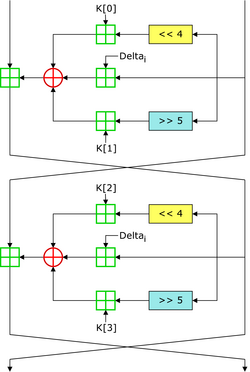
\includegraphics[width=0.4\textwidth]{TEA_InfoBox_Diagram.png}
\caption{TEA one-round (image from wikipedia)}
\label{TEA_InfoBox_Diagram.png}
\end{figure}



\section{design}

\begin{figure}[H]
\centering
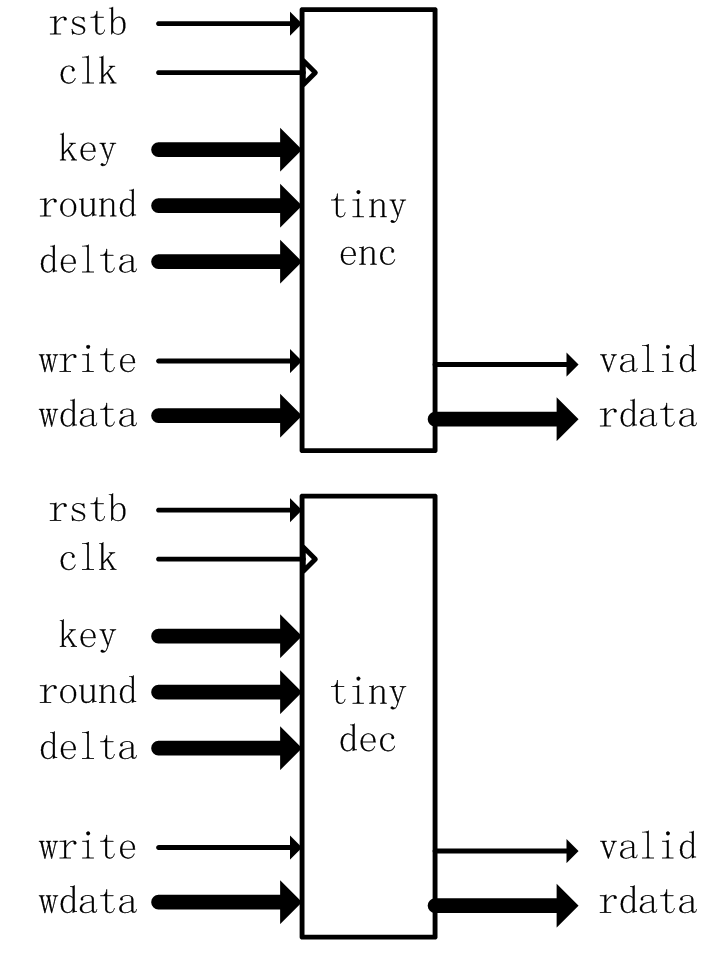
\includegraphics[width=0.5\textwidth]{20250808173800_719x962_scrot.png}
\caption{Ports}
\label{20250808173800_719x962_scrot.png}
\end{figure}



\end{document}
